\documentclass[acmtog]{acmart}
\usepackage{graphicx}
\usepackage{subfigure}
\usepackage{natbib}
\usepackage{listings}
\usepackage{bm}
\parindent=19pt
\definecolor{blve}{rgb}{0.3372549 , 0.61176471, 0.83921569}
\definecolor{gr33n}{rgb}{0.29019608, 0.7372549, 0.64705882}
\makeatletter
\lst@InstallKeywords k{class}{classstyle}\slshape{classstyle}{}ld
\makeatother
\lstset{language=C++,
	basicstyle=\ttfamily,
	keywordstyle=\color{blve}\ttfamily,
	stringstyle=\color{red}\ttfamily,
	commentstyle=\color{magenta}\ttfamily,
	morecomment=[l][\color{magenta}]{\#},
	classstyle = \bfseries\color{gr33n}, 
	tabsize=2
}
\lstset{basicstyle=\ttfamily}

% Title portion
\title{CS171 HW1 assignment:\\ {Exploring OpenGL Programming}} 

\author{Name:\quad Xiaohan WU  \\ student number:\ 2019533093
\\email:\quad wuxh@shanghaitech.edu.cn}

% Document starts
\begin{document}
\maketitle

\vspace*{2 ex}

\section{Introduction}
\qquad In HW1, we are required to realize the mesh reconstruction and rendering using openGL programming with the given object information. The program contains 3 basic parts and 3 optional parts. The first three parts are: 1.Loading mesh objects from files and drawing the meshes.
2.Rendering objects with a Phong lighting model.
3.Manipulating the camera and using the keyboard to control the camera.For the last three parts,we are required to implement a fragment shader to support multiple lights and a geometry shader to change the vertex data utilizing the modern OpenGL properties.
\section{Implementation Details}
\qquad In this section, I will introduce how I implement my program for each part respectively.
\\\indent1.After using 'fin' to load mesh objects from files, I store the vertices information in 'vertices', a vector instance in 'Mesh' class, treating it as VBO. Also,I store the information of how three vertices form a face in 'indices', a vector instance in 'Mesh' class, treating it as EBO.Next, I create a function called 'MeshVAO\_set()' which binds the VBO and EBO to the VAO. After that, we can just use 'draw()' function to draw the meshes.
\\\indent2.For the rendering part, I would like to introduce it with the fragment shader part together. As it is said, I use simplified model-- Phong lighting model to render the object. It contains 3 parts:ambient light, diffuse light and specular light. The complete principle and procedure of those 3 parts are omitted in this paper, and instead I will just list what variables I have calculated in my code--light position, light direction,light color, view direction, object color, fragment position, normal and so on. To make my rendering more realistic, I also introduce attenuation as an improvement. Based on what has mentioned above, realizing multiple lights in fragement shader is relatively easy, which only requires us to add single light effects into a whole.
\\\indent3.Manipulating the camera and using the keyboard to control the camera are not so difficult to implement after understanding the principle of them. For keyboard controlling, I implement a function called 'processInput',which can process what I press on the keyboard and change the camera parameters(including camera position, camera front, camera up) later on. For cursor controlling, I implement 'mouse\_callback' and 'scroll\_call back' functions which change fov, yaw, pitch of the camera, thusing changing the camera front.
\\\indent4.For the geometry shader part, unfortunatelly I don't come up with a good idea, and finally I choose to show off the visualization of the normal vectors of the meshes I render. As the provided 'Shader' class doesn't have the interface of geometry shader, I reimplement this part of code with some improvements. How to visualize the normal vector is also relatively easy, which only requires us to emit the mesh points and points formed by changing the positions of mesh points along their corresponding normal vectors.Finally we can just use 'EndPrimitive()' function to end this part. 
\section{Results}
\qquad Below are the results of my programming work, which present plane, sphere, bunny respectively,shown from Figure (a) to Figure (c). For those objects, I build them under multiple lights, and I also set the background as black so that those models can been represented more clearly.

\begin{figure}[htbp]
	\centering
	\subfigure[Plane]{
		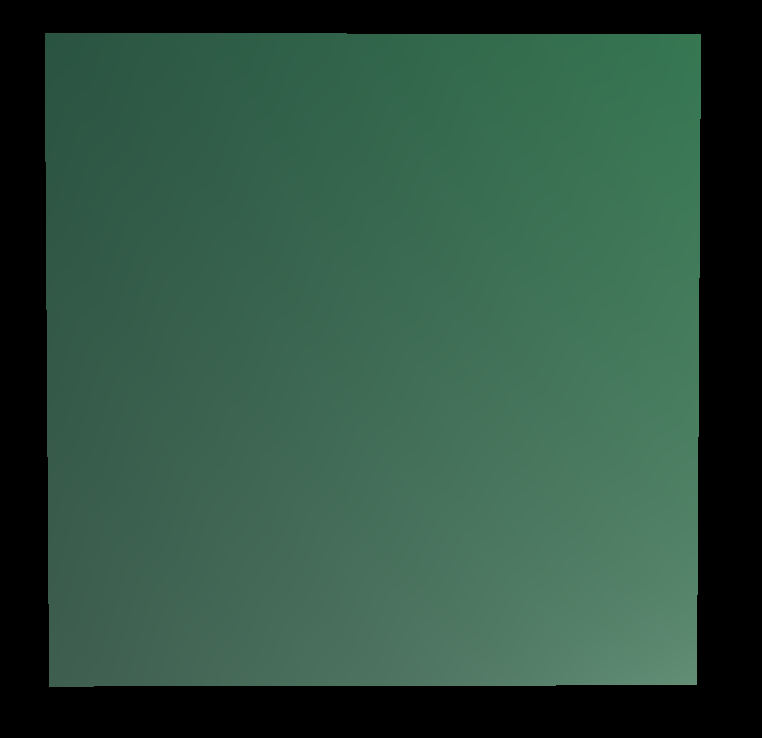
\includegraphics[width=3cm]{plane.PNG}
		%\caption{fig1}
	}
	\quad
	\subfigure[Sphere]{
		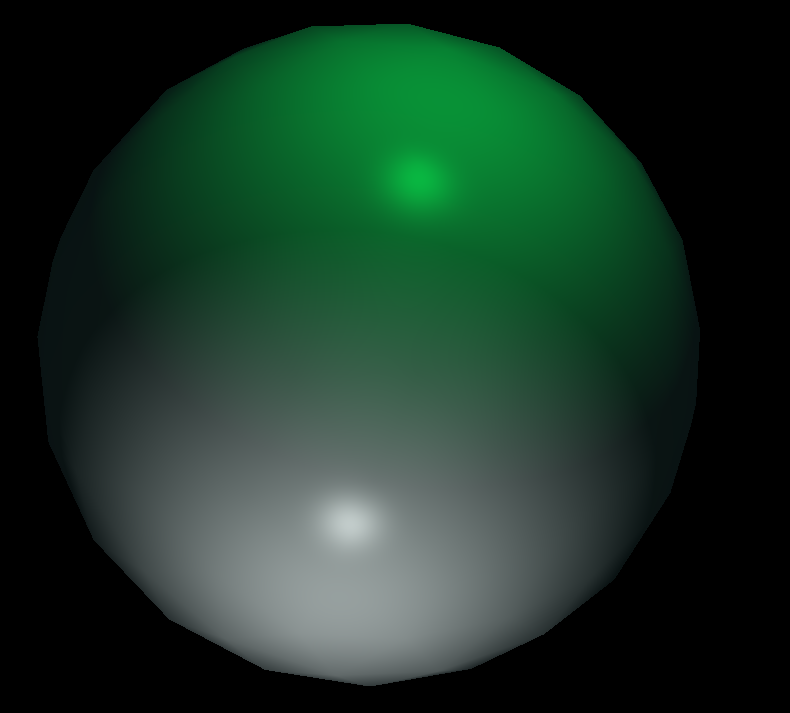
\includegraphics[width=3cm]{sphere.PNG}
	}
	\quad
	\subfigure[Bunny]{
		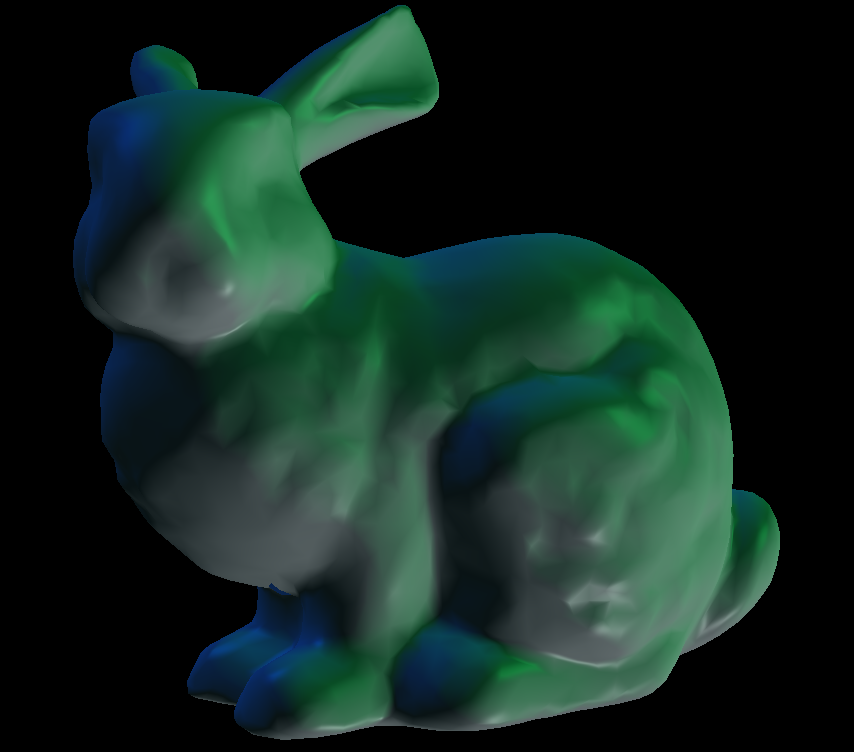
\includegraphics[width=3cm]{bunny.PNG}
	}
	\quad
	\subfigure[Bunny normal visualization]{
		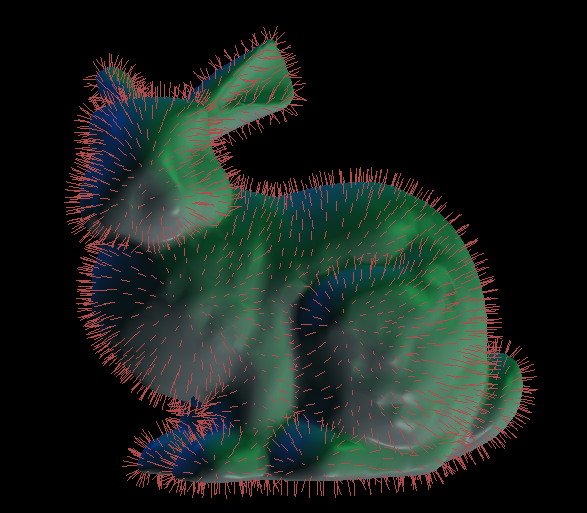
\includegraphics[width=3cm]{bunny_with_geoshader.PNG}
	}
\end{figure}
 Figure (d) shows the visualization of normal vectors of the Bunny, served as a demonstration for the use of geometry shader.
\end{document}
